\documentclass[11pt]{article}
\usepackage{amsmath}
\usepackage{amssymb}
\usepackage{microtype}
\usepackage[english]{babel}
\usepackage[labelsep=period, font=small]{caption}
\usepackage[margin=3cm]{geometry}
\usepackage{graphicx}
\usepackage[utf8]{inputenc}
\usepackage{listings}
\usepackage{mdframed}
\usepackage{float}
\usepackage{wisjab}
\usepackage{xcolor}
\usepackage{subfig}
\usepackage{xcolor}
\frenchspacing
\DisableLigatures[f]{}
\parindent=20pt

\definecolor{medgreen}{rgb}{0.0, 0.6, 0.0}
\definecolor{reddishmauve}{rgb}{0.6, 0.0, 0.3}
\lstset{language=Python, showstringspaces=false, numberfirstline=false, breaklines=true, numbers=left, stepnumber=1, tabsize=4,
basicstyle=\ttfamily, numberstyle=\tiny, commentstyle=\color{medgreen}\rmfamily, stringstyle=\color{reddishmauve}, keywordstyle=\color{blue}}

\DeclareMathOperator*{\argmin}{arg\,min}
\DeclareMathOperator*{\argmax}{arg\,max}
\def\tab{\hspace*{1cm}}

\author{Anonymous [s\,$*******$] and Unknown [s\,$*******$]}
\title{\textsc{\Huge neural networks}\\Assignment II\\[6mm]\large\bf Proof of understanding}

\begin{document}
\maketitle
\section{Recurrent networks}
To understand recurrent neural networks (rnn) we have explored language modeling using tensorflow.  We will be using a rnn that, an input text, will model the probability distribution of the next character in the sequence given a sequence of previous character. The network will then be able to generate new text that will look like the input text. This can help improve speech recognition software. For example if some software is able to only recognize some speech partially, the network could then be used to predict the rest of the speech.\par
For the training data we have used the Sherlock Holmes short stories. The data size is 312 kb. One of the parameters is the sequence length of the network, it is the limit at which the gradients can propagate backwards in time (length of the dependencies). We chose this to be 80 characters because that is the average length of a sentence. Running the network for a few iteration produces the following text: \textit{Res fhe sDiwshy ptovel, hans meutmrlartohci mandnieste ad hs hy tegom, andtLat,}
This is just a sequence of random characters. Increasing the number of iterations to 700 produces the following:
\textit{He she rit; suite attenp the some head was fike whip, Should it wastennwher,"}
\textit{ went while Ferroped not}
We see that words are beginning to form. Now increasing the iterations to 2100
\textit{And I Siberver and one   about to be just had do tell more left in I conversation of anything}
It can now spell words correctly, but the text makes no sense. We did not manage to get any sensible text. But this is still impressive nonetheless. The network had to learn English completely from scratch. Let's see if if we can atleast have some use for this network. We fed the network 5000 baby names. Because the dependancy of babynames is no longer than about 8 characters, this should be a very easy task. The network produced the following:
\textit{ 'Cadoley', 'Candina', 'Carmol', 'Caline', 'Catesse', 'Cammis', 'Caebe', 'Acey', 'Aanda',}\\
\textit{ 'Agged', 'Ensun', 'Ennsus', 'Endi', 'Urabela', 'Erness', 'Erene', 'Emgina', 'Edtor', 'Eedrey',}
\textit{ 'Asalinde', 'Anthorelekely', 'Ande', 'Analda', 'Melcioth', `Mitksa', `Mi'}
We see that the network was able to produce unique names.\par
Because the datasets used weren't large, the hidden layer was kept small so we prevent overfitting. We found that a learning rate of about 0.02 would quickly reduce the training loss. And the sequence length was adjusted accordingly to the data (large sequence length for long term dependency, and short otherwise).
\section{Auto-encoders}
For the auto-encoder we have used the famous MNIST hand written digits. The size of the images are $28\times28=784$ dimensions. The auto-encoder used is stacked with 2 layers and uses tensorflow. The auto-encoder is trained using 256 hidden neurons and the results are fed into an auto-encoder with 128 hidden neurons. The encoder and decoder stages use an sigmoid activation function. The hyperparameters  are the learning rate, epochs and batch size.
\begin{figure}[h]
  \centering
    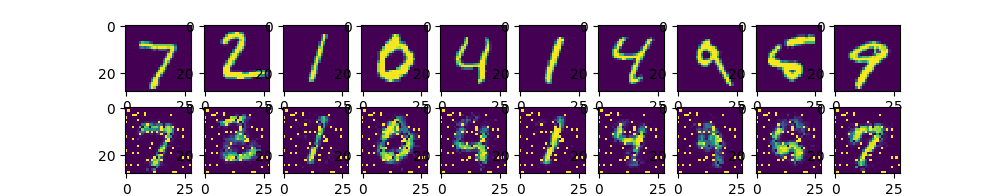
\includegraphics[width=0.8\textwidth]{0,01-15-256-256-128.png}
  \caption{learning rate = 0.01, epochs = 15, batch size = 256, hidden layer 1 = 256, hidden layer 2 = 128}
\end{figure}

Decreasing the batch size should give better results, the auto-encoder should then be able to learn more uncommon features of the data. Decreasing the batch size to 10:

\begin{figure}[h]
  \centering
    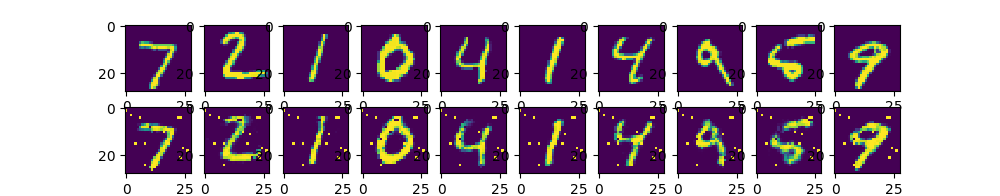
\includegraphics[width=0.8\textwidth]{0,01-15-10-256-128.png}
  \caption{learning rate = 0.01, epochs = 15, batch size = 10, hidden layer 1 = 256, hidden layer 2 = 128}
\end{figure}
The output has significantly improved, however there still are dots spread over the image. This is likely due to the high number of neurons in the hidden layer. If we decrease this the network should force the network to keep components of the input that are useful for reconstructing the common features of the inputs and reject components that are not common features. The network should learn to reject noise from the input. Reducing the hidden layers with a factor half. 
\begin{figure}[h]
  \centering
    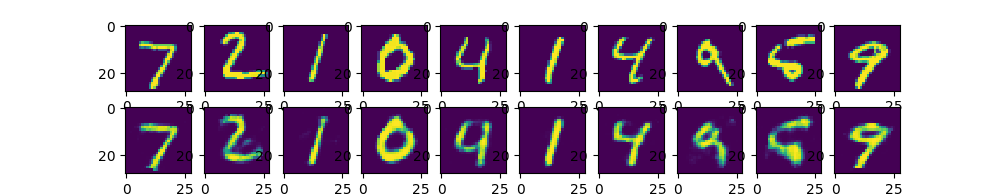
\includegraphics[width=0.8\textwidth]{0,01-15-10-128-56.png}
  \caption{learning rate = 0.01, epochs = 15, batch size = 10, hidden layer 1 = 128, hidden layer 2 = 56}
\end{figure}
The results aren't perfect but still quite good. 
\section{Convolutional networks}
We used a convolutional network on the MNIST handwritten digits data set to classify the images. Since the digits have quit distince features, a cnn should easily be able to distinguish with its filters. A cnn using tensorflow has been used. The hyperparameters are: learning rate and batch size. Using this convolutional network we manually tuned the parameters to find an optimum. 
\begin{figure}[!h]
\centering
\parbox{6cm}{
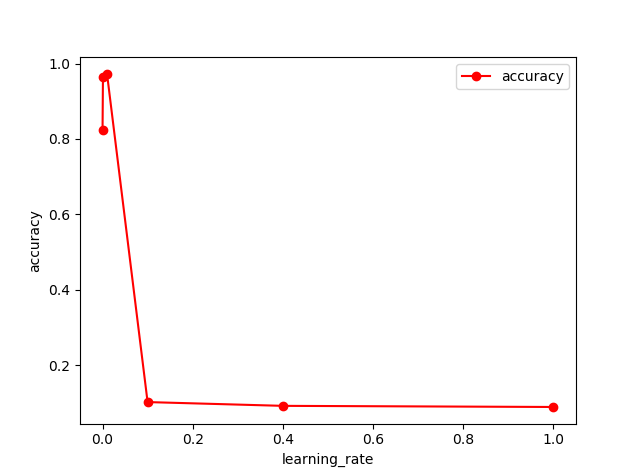
\includegraphics[width=7.5cm]{accuracy_lr.png}
\caption{Accuracy on the test set for varying learning rate. Batch size 128}
\label{fig:2figsA}}
\qquad
\begin{minipage}{6cm}
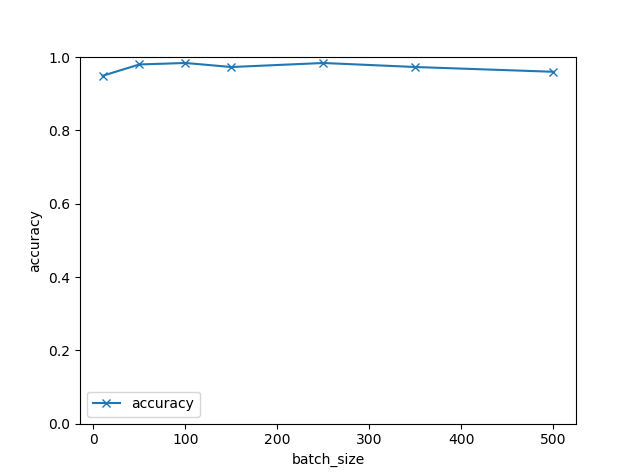
\includegraphics[width=7.5cm]{accuracy_bs.png}
\caption{Accuracy on the test set for varying batch size, learningn rate 0.005}
\label{fig:2figsB}
\end{minipage}
\end{figure}

A learning rate above 0.1 results in low accuracy, around 0.005 the accuracy is 0.98. And it seems that the batch size does not have a large influence on the accuracy. This is due to the fact that a convolution network is able to learn from a single data element due to the convolution layer. Different batch sizes dont factor in its ability to learn well.
\vspace*{\fill}
\begin{thebibliography}{x}
\bibitem{examples}https://github.com/aymericdamien/TensorFlow-Examples
\bibitem{char}https://github.com/sherjilozair/char-rnn-tensorflow
\end{thebibliography}
\end{document}
